%%%%%%%%%%%%%%%%%%%%%%%%%%%%%%%%%%%%%%%%%%%%%%%%%%%%%%%%%%%%
%%  This Beamer template was created by Cameron Bracken.
%%  Anyone can freely use or modify it for any purpose
%%  without attribution.
%%
%%  Last Modified: January 9, 2009
%%

\documentclass[xcolor=x11names,compress]{beamer}

%% General document %%%%%%%%%%%%%%%%%%%%%%%%%%%%%%%%%%
\usepackage{graphicx}
\usepackage[utf8]{inputenc}
\usepackage[T1]{fontenc}
\usepackage[english]{babel}
\usepackage{amsmath,amssymb,amsthm,amsopn}
\usepackage{mathrsfs}
\usepackage{graphicx}
\usepackage{tikz}
\usepackage{array}
\usepackage{makecell}
%\usepackage[top=1cm,bottom=1cm]{geometry}
%\usepackage{listings}
%\usepackage{xcolor}
\usepackage{hyperref}
\hypersetup{
    colorlinks=true,
    linkcolor=blue,
    citecolor=red,
}

\newtheoremstyle{break}%
{}{}%
{\itshape}{}%
{\bfseries}{}%  % Note that final punctuation is omitted.
{\newline}{}

\newtheoremstyle{sc}%
{}{}%
{}{}%
{\scshape}{}%  % Note that final punctuation is omitted.
{\newline}{}

\theoremstyle{break}
\newtheorem{thm}{Theorem}[section]
\newtheorem{lm}[thm]{Lemma}
\newtheorem{prop}[thm]{Proposition}
\newtheorem{cor}[thm]{Corollary}

\theoremstyle{sc}
\newtheorem{exo}{Exercice}

\theoremstyle{definition}
\newtheorem{defi}[thm]{Definition}
\newtheorem{ex}[thm]{Example}

\theoremstyle{remark}
\newtheorem{rem}[thm]{Remark}

% Raccourcis pour les opérateurs mathématiques (les espaces avant-après sont
% modifiés pour mieux rentrer dans les codes mathématiques usuels)
\DeclareMathOperator{\Ker}{Ker}
\DeclareMathOperator{\Id}{Id}
\DeclareMathOperator{\Img}{Im}
\DeclareMathOperator{\Card}{Card}
\DeclareMathOperator{\Vect}{Vect}
\DeclareMathOperator{\Tr}{Tr}
\DeclareMathOperator{\Mod}{mod}
\DeclareMathOperator{\Ord}{Ord}
\DeclareMathOperator{\ppcm}{ppcm}


% Nouvelles commandes
\newcommand{\ps}[2]{\left\langle#1,#2\right\rangle}
\newcommand{\ent}[2]{[\![#1,#2]\!]}
\newcommand{\diff}{\mathop{}\!\mathrm{d}}
\newcommand{\ie}{\emph{i.e. }}
\newcommand{\eg}{\emph{e.g. }}
%%%%%%%%%%%%%%%%%%%%%%%%%%%%%%%%%%%%%%%%%%%%%%%%%%%%%%


%% Beamer Layout %%%%%%%%%%%%%%%%%%%%%%%%%%%%%%%%%%
\useoutertheme[subsection=false,shadow]{miniframes}
\useinnertheme{default}
\usefonttheme{serif}
\usepackage{palatino}
\setbeamertemplate{navigation symbols}{}%remove navigation symbols
\setbeamertemplate{footline}[frame number]


\setbeamerfont{title like}{shape=\scshape}
\setbeamerfont{frametitle}{shape=\scshape}

\setbeamercolor*{lower separation line head}{bg=DeepSkyBlue4} 
% \setbeamercolor*{normal text}{fg=black,bg=white} 
% \setbeamercolor*{alerted text}{fg=red} 
% \setbeamercolor*{example text}{fg=black} 
% \setbeamercolor*{structure}{fg=black} 
%  
\setbeamercolor*{palette tertiary}{fg=black,bg=black!10} 
\setbeamercolor*{palette quaternary}{fg=black,bg=black!10} 
% 
% \renewcommand{\(}{\begin{columns}}
% \renewcommand{\)}{\end{columns}}
% \newcommand{\<}[1]{\begin{column}{#1}}
% \renewcommand{\>}{\end{column}}

\AtBeginSection[]{
  \begin{frame}
  \vfill
  \centering
  \begin{beamercolorbox}[sep=8pt,center,shadow=false,rounded=true]{title}
    \usebeamerfont{title}\secname\par%
  \end{beamercolorbox}
  \vfill
  \end{frame}
}

%%%%%%%%%%%%%%%%%%%%%%%%%%%%%%%%%%%%%%%%%%%%%%%%%%




\begin{document}


%%%%%%%%%%%%%%%%%%%%%%%%%%%%%%%%%%%%%%%%%%%%%%%%%%%%%%
%%%%%%%%%%%%%%%%%%%%%%%%%%%%%%%%%%%%%%%%%%%%%%%%%%%%%%
\begin{frame}
  \title{Discrete logarithm in finite fields of small characteristic}
%\subtitle{SUBTITLE}
  \author{}
\date{\today}
\titlepage
\end{frame}

%%%%%%%%%%%%%%%%%%%%%%%%%%%%%%%%%%%%%%%%%%%%%%%%%%%%%%
%%%%%%%%%%%%%%%%%%%%%%%%%%%%%%%%%%%%%%%%%%%%%%%%%%%%%%
\begin{frame}{Contents}
  \tableofcontents[hideallsubsections]
\end{frame}

%%%%%%%%%%%%%%%%%%%%%%%%%%%%%%%%%%%%%%%%%%%%%%%%%%%%%%
%%%%%%%%%%%%%%%%%%%%%%%%%%%%%%%%%%%%%%%%%%%%%%%%%%%%%%
\section{\scshape Introduction}
\subsection{The discrete logarithm problem}
\begin{frame}{Context}
  \begin{itemize}
    \item $G=\left\langle g \right\rangle$ cyclic group generated by $g$
    \item $N=\Card G$.
    \end{itemize}
  
  We have an \emph{isomorphism}
  \[
    \begin{array}{cccc}
      \exp_g: & (\mathbb{Z}/N\mathbb{Z},+) & \to & (G,\times) \\
      & n & \mapsto & g^n
    \end{array}
  \]

  \begin{itemize}
    \item $\log_g:=\exp_g^{-1}$
   \item Compute $g^n$ from $n$: \textcolor{green}{\bf easy} (polynomial in
     $\log n$)
    \item Compute $n$ from $g^n$: \textcolor{red}{\textbf{hard} (discrete
    logarithm problem)}
  \end{itemize}
\end{frame}

\subsection{Terminology}
\begin{frame}{Definitions}
  Two families of algorithms:
  \begin{itemize}
    \item The \emph{generic} algorithms (complexity:
      $\textcolor{purple}{O(\sqrt N)}$)
    \item The \emph{index calculus} algorithms, using group structure
      \begin{itemize}
        \item from now on: $G=\mathbb{F}_{q^n}^\times$
      \end{itemize}
    \end{itemize}
    Terminology:
    \begin{itemize}
      \item \emph{small characteristic}: $\mathbb{F}_{q^n}$ with $q\ll q^n$
    \item \emph{quasi-polynomial} complexity:
      $\textcolor{purple}{\ell^{O(\log\ell)}}$ where $\ell=\log(q^n)$
      \item \emph{Notation:}
  \end{itemize}
  \[
    \textcolor{purple}{L_N(\alpha) = \exp((c+o(1))(\log N)^\alpha(\log\log
      N)^{1-\alpha})}
  \]

  \begin{center}
    $L_N(0) = (\log N)^{c+o(1)}$ \phantom{blablabla} $
    L_N(1) = N^{c+o(1)}$
  \end{center}

\end{frame}

\subsection{Historical background}
\begin{frame}{Historical background}
  \begin{itemize}
    \item First appearance in \textcolor{blue}{[Diffie, Hellman '76]}
    \item First sub-exponential algorithm in $\mathbb{Z}/p\mathbb{Z}$ \textcolor{blue}{[Adleman '79]}:
      $\textcolor{purple}{L_N(1/2)}$
    \item Between 1984 and 2006: algorithms in $\textcolor{purple}{L_N(1/3)}$
\end{itemize}
 And more recently, in finite fields of small characteristic:
  \begin{itemize}
    \item New algorithm with $\textcolor{purple}{L_N(1/4)}$ complexity
      \textcolor{blue}{[Joux '13]}
    \item \emph{Quasi-polynomial} algorithm \textcolor{blue}{[Barbulescu,
      Gaudry, Joux, Thomé '14]}
    \item Second quasi-polynomial algorithm \textcolor{blue}{[Granger,
      Kleinjung, Zumbrägel '14]}
  \end{itemize}
\end{frame}
\begin{frame}{Some practical records}
  \begin{tabular}[here]{lllll}
    Date & Field & Bitsize & Algorithm & Authors \\
    \hline
    & & & & \\
    2013/02 & $2^{1778}$ & $1778$ & $L(1/4)$ & Joux \\
    2013/02 & $2^{1991}$ & $1991$ & GKZ & \makecell[lc]{Göloglu, Granger, \\ McGuire,
    Zumbrägel} \\
    2013/05 & $2^{6168}$ & $6168$ & $L(1/4)$ & Joux \\
    2014/01 & $3^{6\cdot137}$ & $1303$ & $L(1/4)$, GKZ & \makecell[lc]{Adj,
    Menezes, Oliveira, \\ Rodr\'iguez-Henr\'iquez}\\
    2014/01 & $2^{9234}$ & $9234$ & $L(1/4)$, GKZ & \makecell[lc]{Granger,
    Kleinjung,\\Zumbrägel}\\
    2014 & $3^{6\cdot509}$ & $4034$ & $L(1/4)$, GKZ & \makecell[lc]{Adj,
    Menezes, Oliveira, \\ Rodr\'iguez-Henr\'iquez}\\
  \end{tabular}
  \begin{itemize}
    \item Runtime of the last computation: $220$ CPU years 
  \end{itemize}
\end{frame}

\section{\scshape Index calculus}
\subsection{Overview}
\begin{frame}{Overview}
  \emph{Goal:} find $\log_g(h)$ 
  \begin{enumerate}
    \item[0.] first choose $F\subset
  G$ with $\left\langle F \right\rangle = G$
    \item find multiplicative relations between elements in $F$
    \item solve the associated linear system for $\{ \log_g(f)\;|\;f\in F\}$
    \item express $h$ as a product of elements in $F$
  \end{enumerate}
  Steps $1$ and $3$ depend on the structure of the finite field, different
  fields give different complexities for the index calculus.
\end{frame}

\subsection{An example}
\begin{frame}{An example: Adleman}
  \emph{Context:}
  \begin{itemize}
    \item $G = \mathbb{F}_p^\times = \langle g\rangle$ for a prime $p$ and $N = |G| = p-1$
    \item $F = \left\{\, f \;|\; f \leq B,\; f \text{ prime}
    \right\}$ for a chosen integer $B$
  \end{itemize}

  \emph{Step 1: relations generation}
  \begin{itemize}
    \item randomly choose $e\in \mathbb{Z}/N\mathbb{Z}$
    \item test if $g^e$ is $B$-smooth
    \item if it is the case, it yields a relation in $G$:
      \[ 
        g^e = \prod_{f\in F}f^{e_f}, e_f\in \mathbb{N}
      \]
      that can be written
      \[
        e = \sum_{f\in F}e_f\log_g(f).
      \]
  \end{itemize}
\end{frame}

\begin{frame}{An example}
  \emph{Step 2: linear algebra:} solve the linear system
  
  \emph{Step 3: express $h$ as a function of the elements in $F$:}
  \begin{itemize}
     \item randomly choose $e\in \mathbb{Z}/N\mathbb{Z}$
    \item test if $hg^e$ is $B$-smooth
    \item if it is the case, it yields a relation:
     \[
      \log_g(h) = \sum_{f\in F}e_f\log_g(f) - e
      \]
  \end{itemize}

 Depends on $B$:
  \begin{itemize}
    \item $B$ large: easier to find relations
    \item $B$ large: need more relations to solve the system
  \end{itemize}
  Complexity: $\textcolor{purple}{L_N(1/2)}$

\end{frame}

\section{\scshape Quasi-polynomial algorithms} 
\subsection{Main ideas}
\begin{frame}{Comparison with Adleman}
  \begin{center}
  \begin{tabular}[here]{lcc}
  Algorithm  & Adleman & Quasi-polynomial \\
  \hline
  & & \\
  Field & $\mathbb{F}_p=\mathbb{Z}/p\mathbb{Z}$ & $\mathbb{F}_{q^n}\cong \mathbb{F}_q[X]/(P)$ \\
  Elements repr. by & integers & polynomials \\
  Subset $F\subset G$ & primes $\leq B$ & irreducibles of degree $\leq B$ \\
  \end{tabular}
  \end{center}

  \emph{Goal:} find polynomials that factor into irreducible polynomials of small degree.
\end{frame}

\begin{frame}{Main ideas}
  \begin{enumerate}
    \item Use homographies:
      \begin{itemize}
        \item $Q$ polynomial that factors nicely
        \item $m(X) = \frac{aX+b}{cX+d}$ an homography
      \end{itemize}
      $m\cdot Q = (cX+d)^{\deg Q}Q(\frac{aX+b}{cX+d})$ factors nicely too
      \newline
    \item Use Idea $1$ on $X^q-X$ (factors into linear polynomials)
      \newline
    \item Take advantage of the freedom for the defining polynomial $P$ of
      $\mathbb{F}_{q^n}=\mathbb{F}_q[X]/(P)$ to simplify $X^q$
      \begin{itemize}
        \item We choose $P\;|\;h_1X^q-h_0$ with $h_0, h_1$ polynomials of small
          degree (existence of $h_0, h_1$
          \textcolor{violet}{\textbf{heuristic}})
        \item We obtain $X^q \equiv \frac{h_0(X)}{h_1(X)}$ in
          $\mathbb{F}_q[X]/(P)$
      \end{itemize}
  \end{enumerate}
\end{frame}

\begin{frame}{Quasi-polynomial complexity}
  \emph{Goal:} $\mathbb{F}_{q^n}$ field, find $\log Q$ for $Q\in
  \mathbb{F}_{q^n}$ 
  \begin{itemize}
    \item not able to express $\log Q$ as elements in $F$ in one step 
  \end{itemize}
\begin{prop}
  Let $Q$ be an element of a field $\mathbb{F}_{q^n}$. There exists a
  \textcolor{violet}{\textbf{heuristic}} algorithm whose complexity is polynomial in
  $\ell=\log(q^n)$ which returns an expression of $\log Q$ as a linear combination of
  at most $\mathcal N$ logarithms $\log Q_j$ with $\deg Q_j\leq \lceil
  \frac{1}{2}\deg Q\rceil$.
\end{prop}
\begin{itemize}
  \item Barbulescu, Gaudry, Joux, Thomé: $n$ even and $\mathcal
    N=O(q^2 \frac{n}{2})$
  \item Granger, Kleinjung, Zumbrägel: $\mathcal N =
    q+2$
\end{itemize}
\end{frame}

\begin{frame}{The descent}
  \begin{figure}
  \centering
  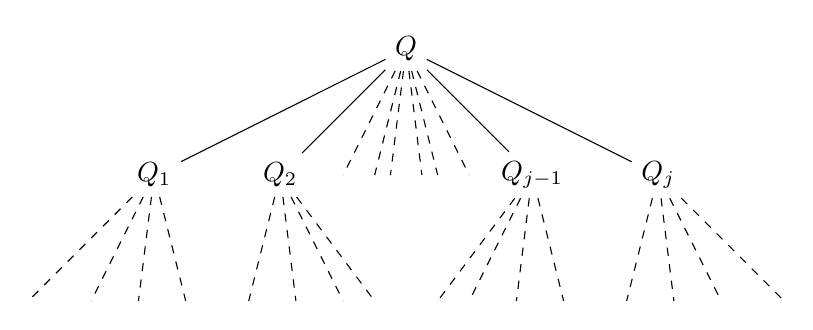
\begin{tikzpicture}[scale=0.8]
    \node (Q) at (0,0) {$Q$};  

    \node (Q1) at (-4, -2) {$Q_1$}; 
    \node (Q2) at (-2, -2) {$Q_2$}; 
    \node (Q3) at (2, -2) {$Q_{j-1}$}; 
    \node (Q4) at (4, -2) {$Q_j$}; 

    \draw (Q) -- (Q1);
    \draw (Q) -- (Q2);
    \draw (Q) -- (Q3);
    \draw (Q) -- (Q4);

    \draw[dashed] (Q) -- (-1, -2);
    \draw[dashed] (Q) -- (1, -2);
    \draw[dashed] (Q) -- (-0.5, -2);
    \draw[dashed] (Q) -- (0.5, -2);
    \draw[dashed] (Q) -- (-0.25, -2);
    \draw[dashed] (Q) -- (0.25, -2);

    \draw[dashed] (Q1) -- (-6, -4);
    \draw[dashed] (Q1) -- (-5, -4);
    \draw[dashed] (Q1) -- (-4.25, -4);
    \draw[dashed] (Q1) -- (-3.5, -4);

    \draw[dashed] (Q2) -- (-0.5, -4);
    \draw[dashed] (Q2) -- (-1, -4);
    \draw[dashed] (Q2) -- (-2.5, -4);
    \draw[dashed] (Q2) -- (-1.75, -4);

    \draw[dashed] (Q3) -- (0.5, -4);
    \draw[dashed] (Q3) -- (1, -4);
    \draw[dashed] (Q3) -- (2.5, -4);
    \draw[dashed] (Q3) -- (1.75, -4);


    \draw[dashed] (Q4) -- (3.5, -4);
    \draw[dashed] (Q4) -- (4.25, -4);
    \draw[dashed] (Q4) -- (5, -4);
    \draw[dashed] (Q4) -- (6, -4);
  \end{tikzpicture}
  \caption{The descent tree}
\end{figure}
\begin{itemize}
  \item Each node: one application of the Proposition (polynomial time
    algorithm), \textcolor{violet}{number of nodes $=\text{ arity}^{\text{depth}}$}
  \item $\text{arity}=\mathcal N = O(\ell^{O(1)})$, $\text{depth}=O(\log(\ell))$
  \item Complexity: \textcolor{purple}{$\ell^{O(\log \ell)}$}
\end{itemize}
\end{frame}

\subsection{Barbulescu, Gaudry, Joux and Thomé algorithm}

\begin{frame}{Barbulescu, Gaudry, Joux and Thomé}
  \emph{Context:}
  \begin{itemize}
    \item $\mathbb{K}=\mathbb{F}_{q^{2m}}=\mathbb{F}_{q^2}[X]/(P)$ with $P$ irreducible
      polynomial of degree $m$ dividing $h_1X^q-h_0, \deg h_i\leq 2$.
    \item $F=\left\{  \text{degree one polynomials}\right\}\bigcup\left\{ h_1
      \right\}$ 
\end{itemize}
\emph{Descent:} based on the equation
 \begin{equation}
   X^qY - XY^q = Y\prod_{a\in\mathbb{F}_q}(X - aY)
   \label{keyeq}
 \end{equation}

  \begin{itemize}
   \item Substitute $X$ by $aQ + b$ and $Y$ by $cQ + d$ in (\ref{keyeq})
   \item Combine these equations to express $Q$ as polynomials of degree $\leq
     \lceil\frac{1}{2}\deg Q\rceil$ (\textcolor{violet}{\textbf{linear
     algebra}})
\end{itemize}
\end{frame}

\subsection{Granger, Kleinjung and Zumbrägel algorithm}

\begin{frame}{Granger, Kleinjung and Zumbrägel}
  \emph{Context:}
  \begin{itemize}
    \item $\mathbb{K}=\mathbb{F}_{q^n} = \mathbb{F}_q[X]/(P)$ with
  $P$ irreducible polynomial of degree $n$ dividing $h_1X^q-h_0$.
  \end{itemize}
  \emph{Descent:} $Q\in\mathbb{F}_q[X]$ irreducible of degree $2d$
  \begin{itemize}
    \item Factor $Q$ in $\mathbb{F}_{q^d}$: $Q=\prod_{j=0}^{d-1} Q_j$ with $\deg
      Q_j=2$
    \item Express each $Q_j$ as $q+2$ linear polynomials $R_{j,k}$ in
      $\mathbb{F}_{q^d}[X]$ (this is called ``on-the-fly'' elimination)
    \item $Q$ is expressed as $q+2$ polynomials $N_k = \prod_{j=0}^{d-1}R_{j,k}$
  \end{itemize}
  \emph{Fact:} The polynomials $N_k$ are of degree $d$ in $\mathbb{F}_{q}[X]$
  (not $\mathbb{F}_{q^d}[X]$).
\end{frame}

\begin{frame}{``On the fly'' elimination}
  \emph{Input:}
  \begin{itemize}
    \item $Q\in \mathbb{F}_{q^m}[X]$ and $\deg Q = 2$
  \end{itemize}
  \emph{Output:}
  \begin{itemize}
    \item $Q\leadsto q+2$ polynomials $Q_i$ with $\deg Q_i = 1$ and $Q_i\in
      \mathbb{F}_{q^m}[X]$
  \end{itemize}

  \emph{Ideas}
  \begin{itemize}
    \item Find $(a, b, c)$ such that
      \begin{enumerate}
        \item $\Delta = X^{q+1}+aX^q+bX+c$ splits into linear factors in $\mathbb{F}_{q^m}[X]$
        \item $Q\;|\; (X+a)h_0 + (bX+c)h_1$ (degree $3$)
      \end{enumerate}
      (can be reduced to \textcolor{violet}{\textbf{root finding}})
    \item $ \Delta = \frac{1}{h_1}((X+a)h_0 + (bX+c)h_1)\mod P $
    \item $ h_1\Delta=QL \mod P$
      
  \end{itemize}
\end{frame}

\begin{frame}{Experimental results}
  \emph{Implementation in Julia (based on Nemo/Flint):}
\begin{center}
  \begin{tabular}[here]{lcc}
  Algorithm  & BGJT & GKZ \\
    \hline
    & & \\
    Bottleneck & linear algebra & root finding \\
    arity ($\mathbb{F}_{17^{2\cdot17}}$) & $794$ & $291$ \\
    descent runtime ($\mathbb{F}_{17^{2\cdot17}}$) (seconds) & $9.6$ & $34$ \\
    arity ($\mathbb{F}_{23^{2\cdot23}}$) & $1477$ & $531$ \\
    descent runtime ($\mathbb{F}_{23^{2\cdot23}}$) (seconds) & $80$ & $140$ \\
    arity ($\mathbb{F}_{29^{2\cdot29}}$) & $2360$ & $843$ \\
    descent runtime ($\mathbb{F}_{29^{2\cdot29}}$) (seconds) & $570$ & $400$ \\
  \end{tabular}
\end{center}

  \emph{Open problems:}
  \begin{itemize}
    \item practical improvements
    \item proofs of heuristics
    \item polynomial (heuristic) algorithm
  \end{itemize}

\end{frame}

%%%%%%%%%%%%%%%%%%%%%%%%%%%%%%%%%%%%%%%%%%%%%%%%%%%%%%
%%%%%%%%%%%%%%%%%%%%%%%%%%%%%%%%%%%%%%%%%%%%%%%%%%%%%%
\end{document}
